\documentclass[journal, a4paper]{IEEEtran}
\usepackage{graphicx}   
\usepackage{url}        
\usepackage{amsmath, verbatim}   
\usepackage[brazil]{babel}
\usepackage[utf8]{inputenc, color}
\usepackage[T1]{fontenc}
\usepackage{float}
% Your document starts here!
\begin{document}

% Define document title and author
	\title{Relatório 01 - Fonte Regulada Simples}
	\author{Arthur Pimentel e Matheus Farias
	%\thanks{Advisor: Dipl.--Ing.~Firstname Lastname, Lehrstuhl f\"ur Nachrichtentechnik, TUM, WS 2050/2051.}
    }
	%\markboth{Hauptseminar Digitale Kommunikationssysteme}{}
	\maketitle

% Write abstract here
%\begin{abstract}
%	The short abstract (50-80 words) is intended to give the reader an overview of the work.
%\end{abstract}

% Each section begins with a \section{title} command
\section{Simulação}
	% \PARstart{}{} creates a tall first letter for this first paragraph
	   
    \subsection{Circuito 1}    
    Inicialmente, simulou-se, usando o software LTspiceIV, o circuito da Figura \ref{circuito1}. Em seguida, preencheu-se a segunda e terceira colunas da Tabela \ref{Tabela1}.
    
    \begin{figure}[H]
		\begin{center}
		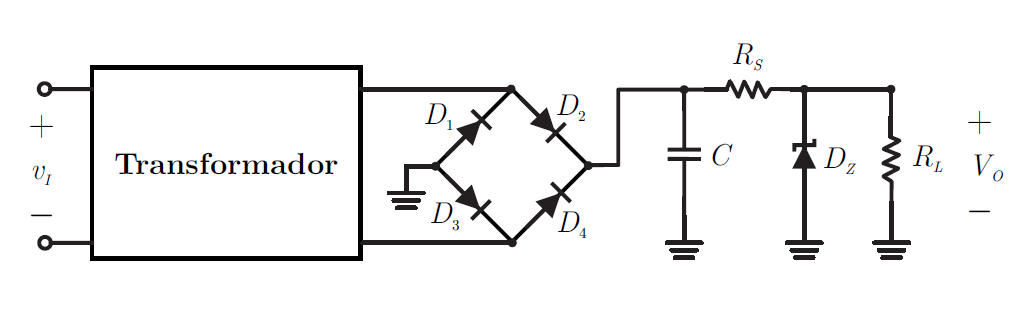
\includegraphics[width=\columnwidth]{Figura_1.PNG}
		\caption{Diagrama de circuito de uma fonte de tensão regulada utilizando o diodo zener.}
		\label{circuito1}
		\end{center}
	\end{figure}
    
    \begin{figure}[H]
		\begin{center}
		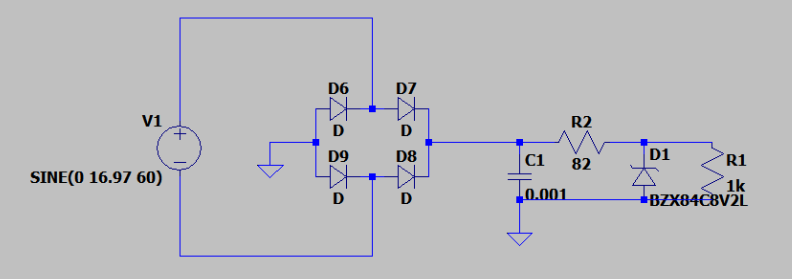
\includegraphics[width=\columnwidth]{Simulacao1.PNG}
		\caption{Simulção do circuito da Figura \ref{circuito1}.}
		\label{simulação1}
		\end{center}
	\end{figure}  

	Com R\textsubscript{L} = 1 k$\Omega$, mede-se o valor médio da tensão e a tensão de \textit{ripple} (V\textsubscript{$r$}) sobre C e sobre R\textsubscript{L}. O resultados são exibidos nas Figuras \ref{V_capacitor}, \ref{V_capacitor_ripple}, \ref{V_resistor} e \ref{V_resistor_ripple}.
    
     \begin{figure}[H]
		\begin{center}
		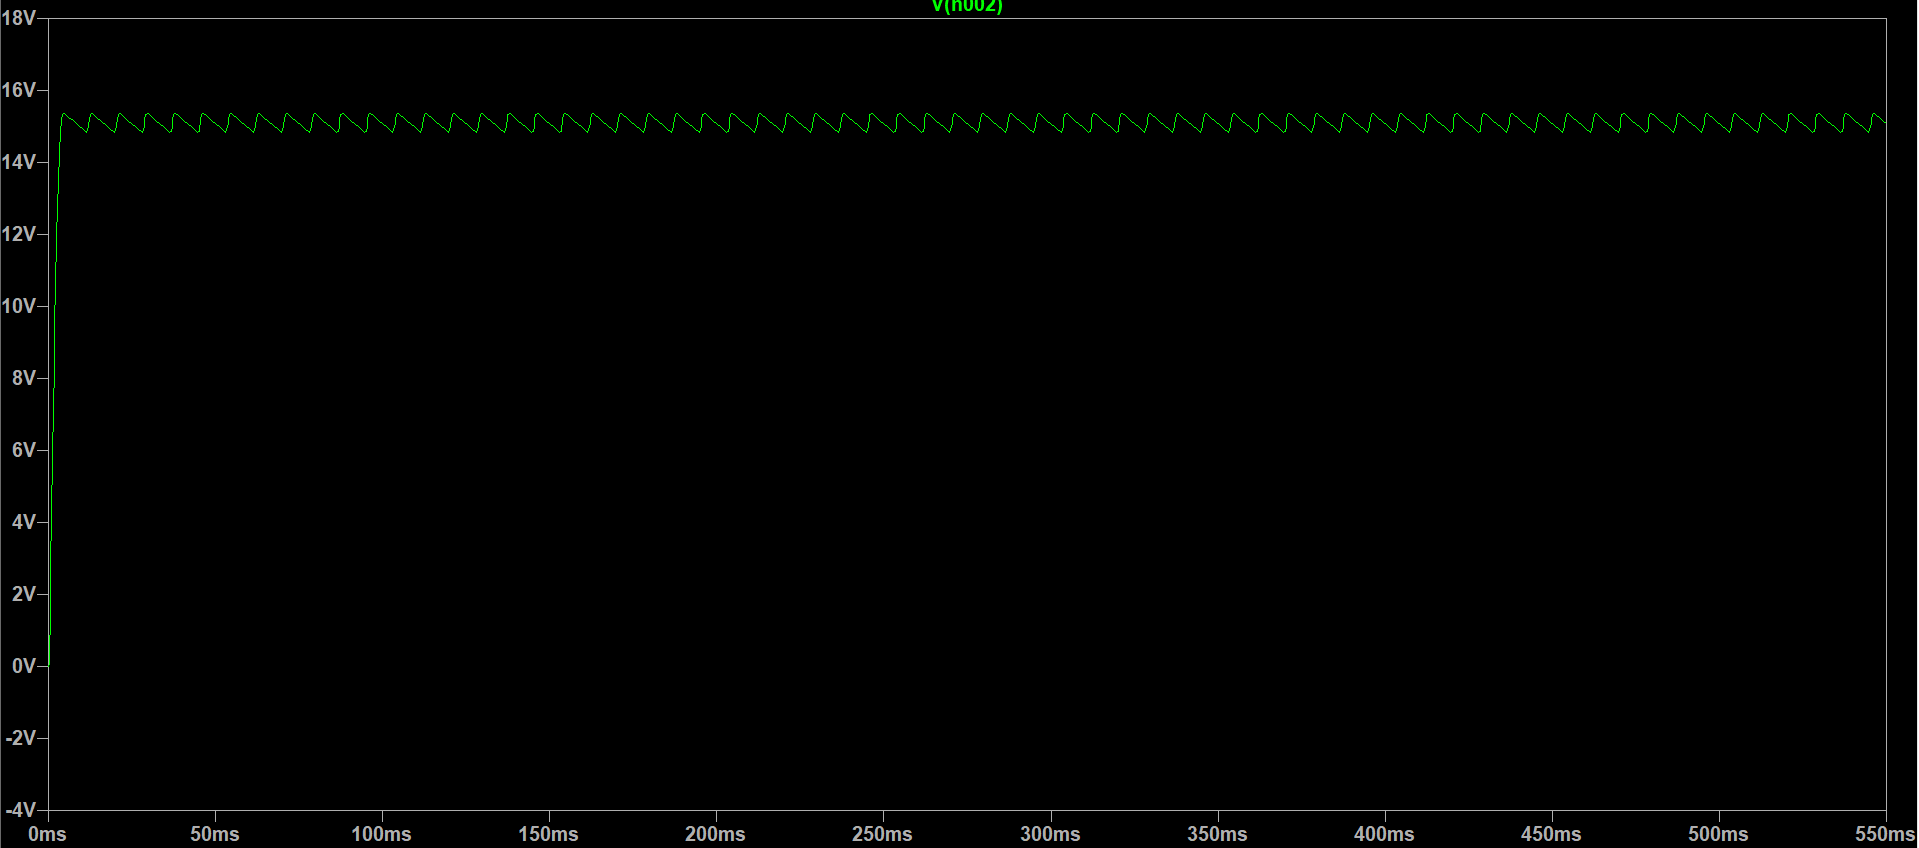
\includegraphics[width=\columnwidth]{circuito1_tensao_capacitor_1.PNG}
		\caption{Tensão média mais o efeito de \textit{ripple} sobre o capacitor da Figura \ref{circuito1}.}
		\label{V_capacitor}
		\end{center}
	\end{figure}
    
     \begin{figure}[H]
		\begin{center}
		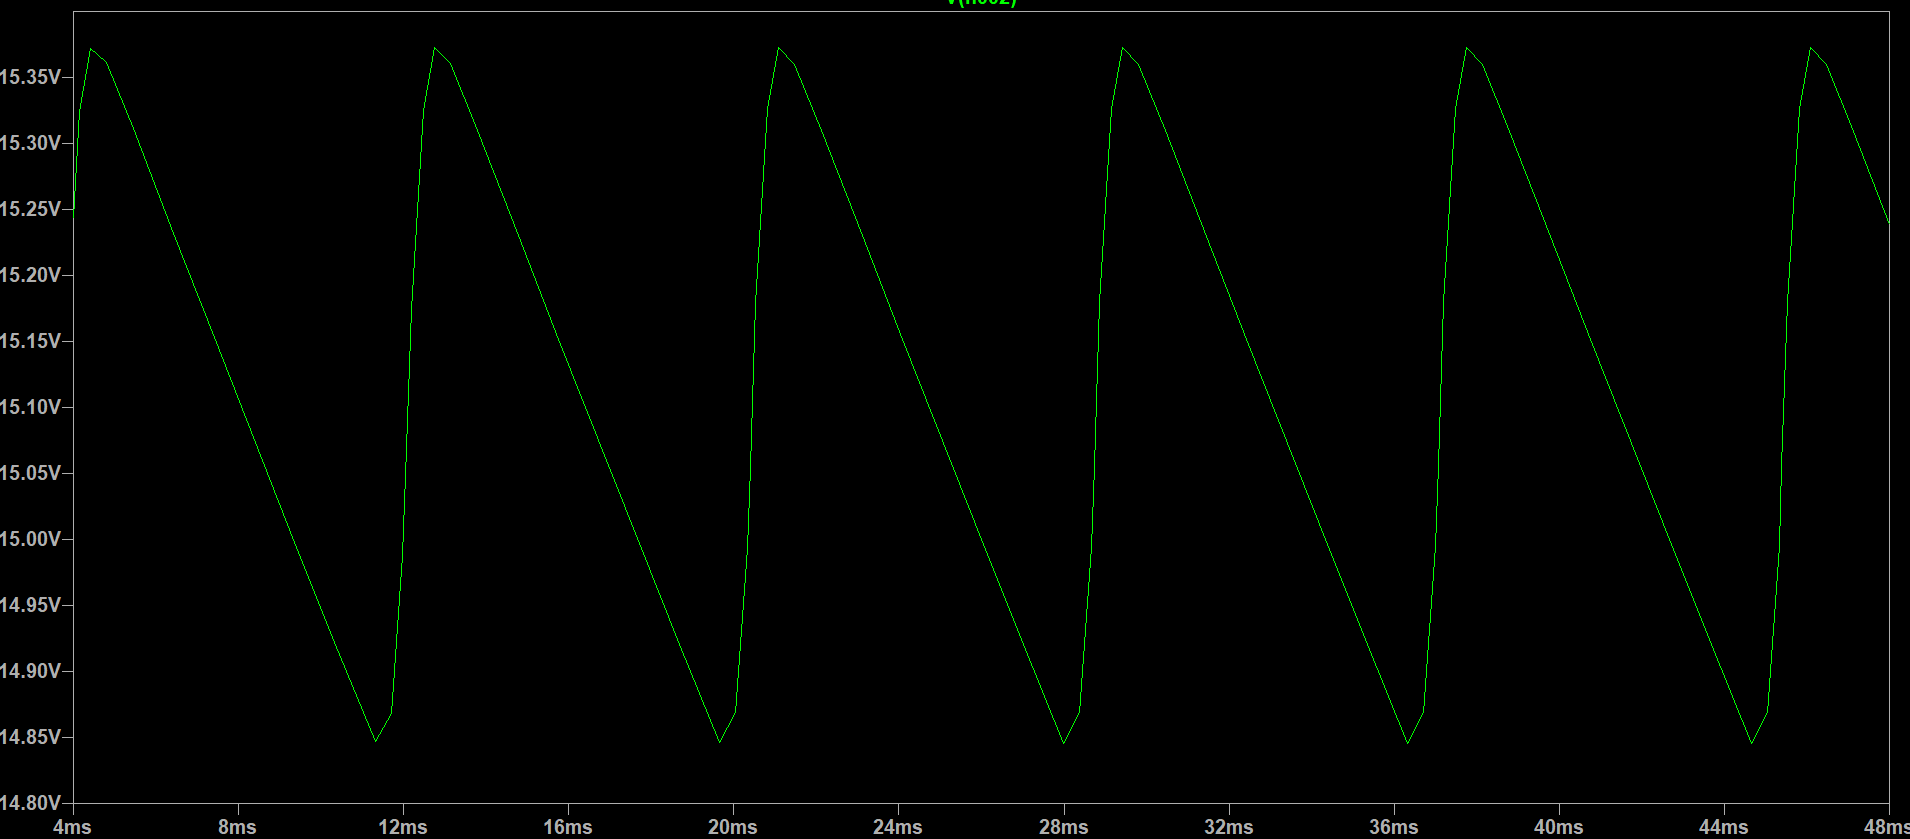
\includegraphics[width=\columnwidth]{circuito1_tensao_capacitor_2.PNG}
		\caption{Observação mais detalhada do efeito de \textit{ripple} sobre o capacitor da Figura \ref{circuito1}.}
		\label{V_capacitor_ripple}
		\end{center}
	\end{figure}
    
     \begin{figure}[H]
		\begin{center}
		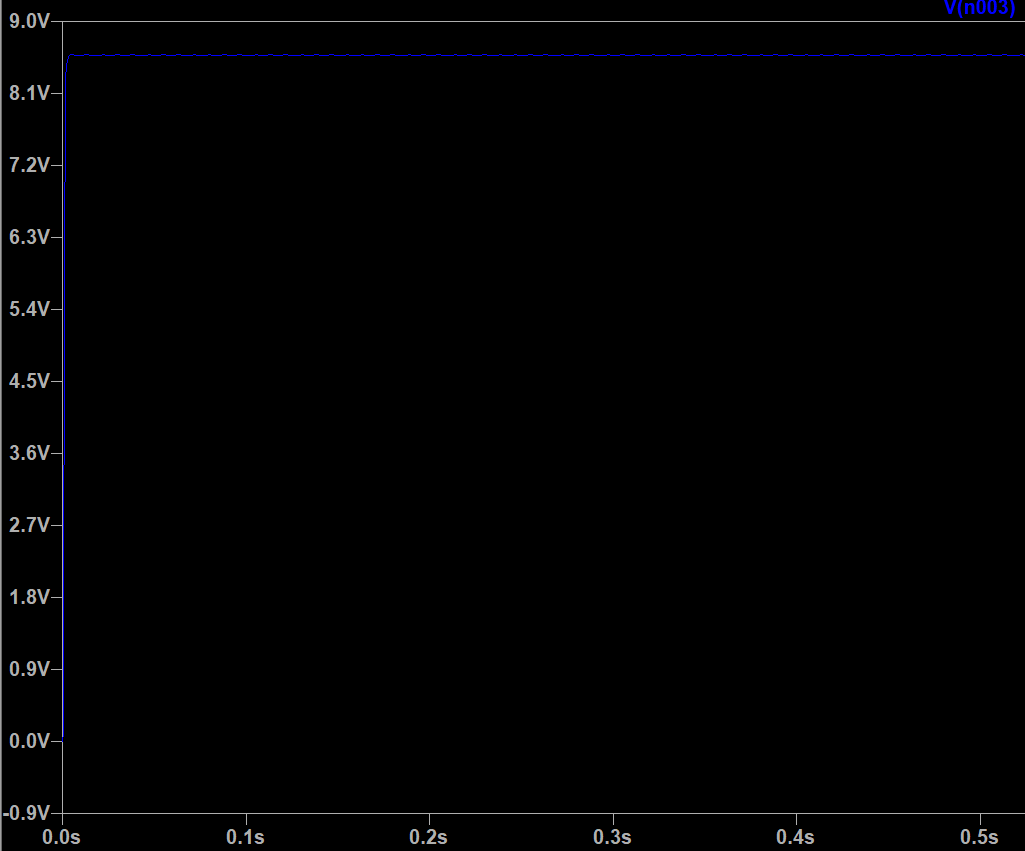
\includegraphics[width=\columnwidth]{circuito1_tensao_resistor_1.PNG}
		\caption{Tensão média mais o efeito de \textit{ripple} sobre o resistor da Figura \ref{circuito1}.}
		\label{V_resistor}
		\end{center}
	\end{figure}
    
     \begin{figure}[H]
		\begin{center}
		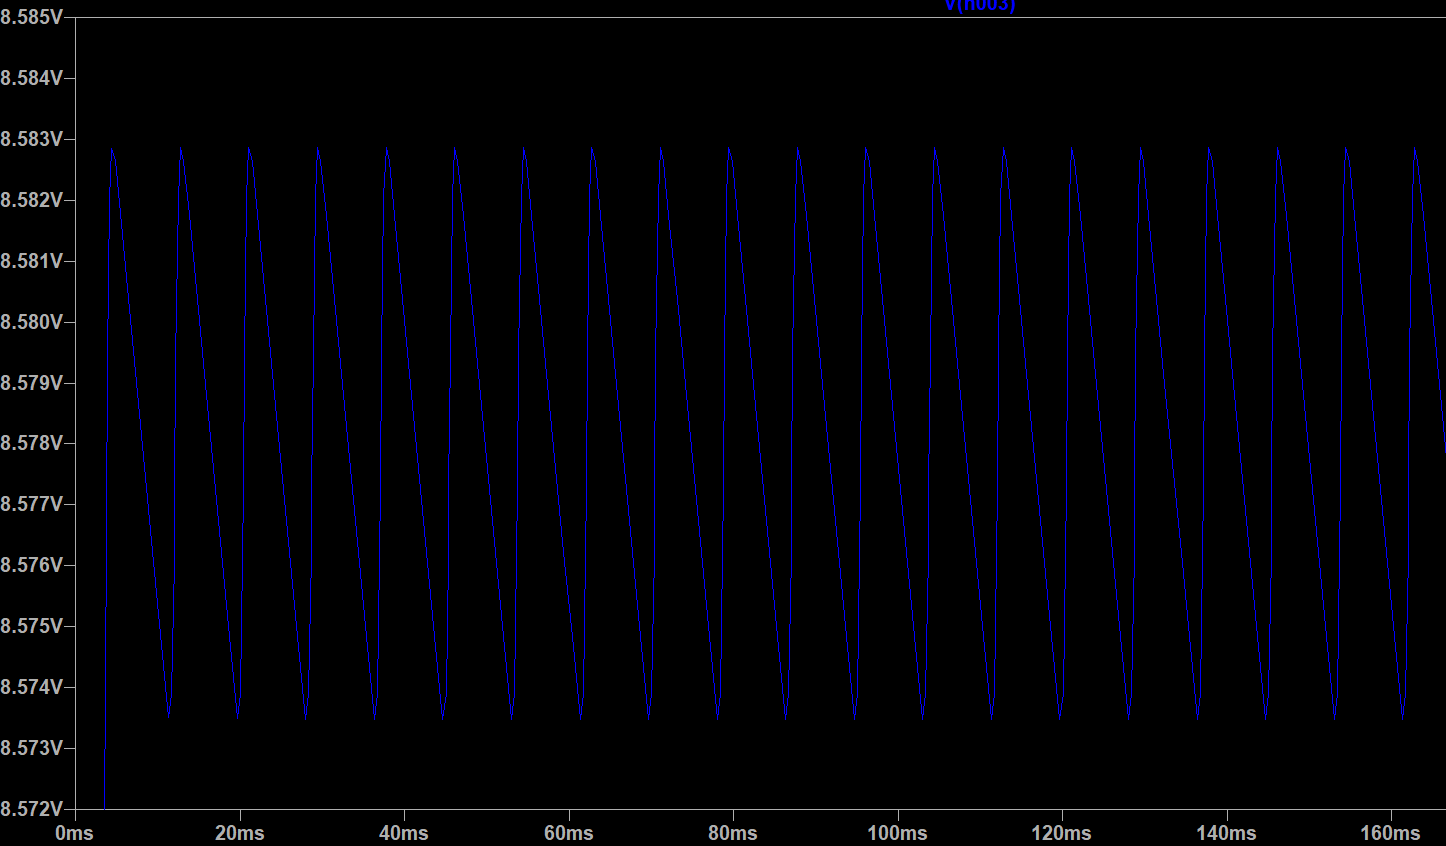
\includegraphics[width=\columnwidth]{circuito1_tensao_resistor_2.PNG}
		\caption{Observação mais detalhada do efeito de \textit{ripple} sobre o resistor da Figura \ref{circuito1}.}
		\label{V_resistor_ripple}
		\end{center}
	\end{figure}
    
    \subsection{Circuito 2}
    Posteriormente, simulou-se, o circuito da Figura \ref{circuito2}.
     
     \begin{figure}[H]
		\begin{center}
		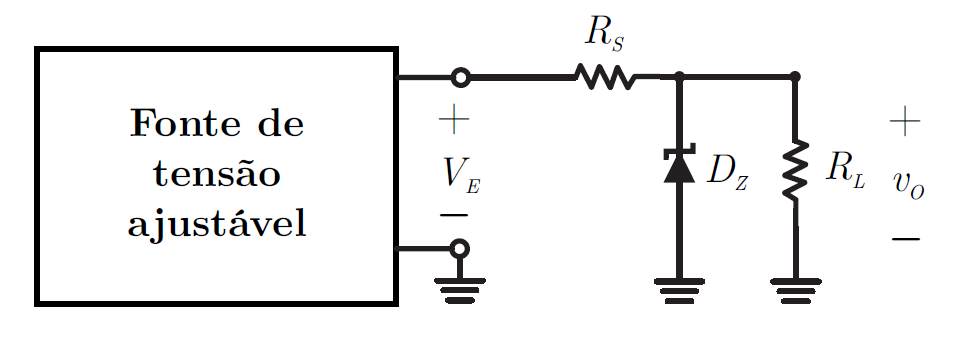
\includegraphics[width=\columnwidth]{Figura_2.PNG}
		\caption{Circuito para o cálculo de V\textsubscript{E(min)}, V\textsubscript{E(max)} e R\textsubscript{L(min)}.}
		\label{circuito2}
		\end{center}
	\end{figure}
    
    \begin{figure}[H]
		\begin{center}
		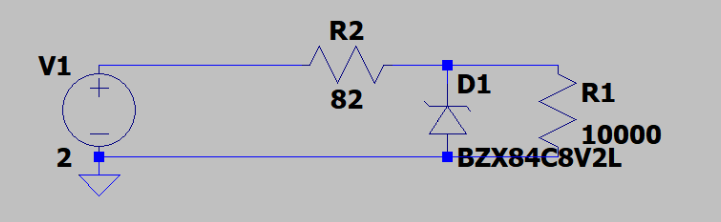
\includegraphics[width=\columnwidth]{Simulacao2.PNG}
		\caption{Simulção do circuito da Figura \ref{circuito2}.}
		\label{simulação2}
		\end{center}
	\end{figure}
    
    Com R\textsubscript{S} = 82$\Omega$, o diodo zener de 8,2 V e R\textsubscript{L} = 1 k$\Omega$, preencheu-se a segunda coluna da Tabela \ref{Tabela2}.








\section{Laboratório}
	\subsection{Circuito 1}
    Monta-se o circuito da Figura \ref{circuito1} e, com o auxílio do multímetro, mede-se os valores de V\textsubscript{0}. Em seguida, preenche-se a Tabela \ref{Tabela1}.

	\begin{table}[H]
		\begin{center}
		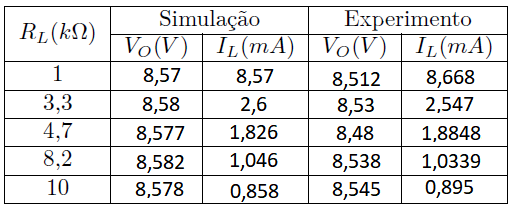
\includegraphics[width=\columnwidth]{Tabela1.png}
		\caption{Valores simulados e experimentais da tensão de saída de V\textsubscript{0} e da corrente na carga I\textsubscript{L} para diferentes valores de R\textsubscript{L} .}
		\label{Tabela1}
		\end{center}
	\end{table}
    
    Com C = 1000 $\mu$F, R\textsubscript{S} = 82 $\Omega$, o diodo zener de 8,2 V e R\textsubscript{L} = 1 k$\Omega$. Usa-se o osciloscópio para medir a tensão sobre C e sobre R\textsubscript{L} assim como o valor de \textit{ripple}. O resultado dessas medições podem ser vistos nas Figuras \ref{scope_capacitor} e \ref{scope_resistor}.
    
     \begin{figure}[H]
		\begin{center}
		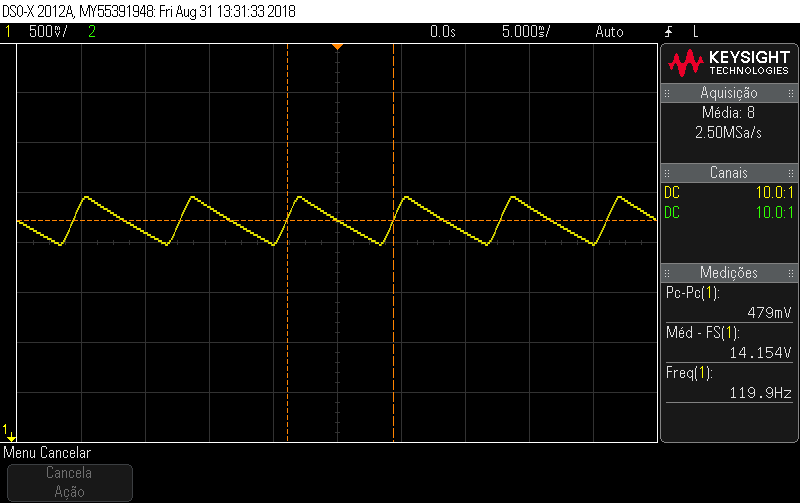
\includegraphics[width=\columnwidth]{scope_1_capacitor.png}
		\caption{Tensão com efeito de \textit{ripple} sobre o capacitor.}
		\label{scope_capacitor}
		\end{center}
	\end{figure}
    
    \begin{figure}[H]
		\begin{center}
		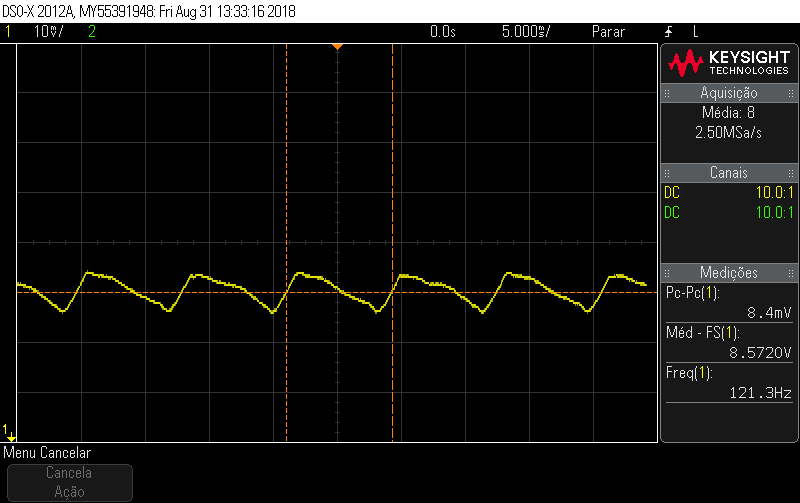
\includegraphics[width=\columnwidth]{scope_2_resistor.png}
		\caption{Tensão com efeito de \textit{ripple} sobre o resistor.}
		\label{scope_resistor}
		\end{center}
	\end{figure}

	\subsection{Circuito 2}
    
	     Monta-se o circuito da Figura \ref{circuito2} e, com o auxílio do multímetro, mede-se os valores de V\textsubscript{0}. Em seguida, preenche-se a Tabela \ref{Tabela2}.

	\begin{table}[H]
		\begin{center}
		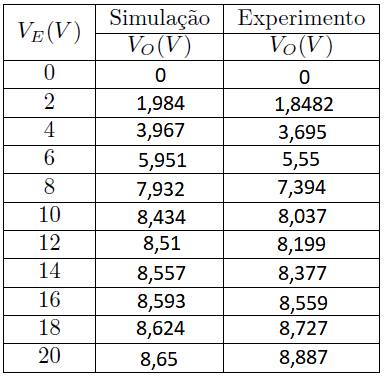
\includegraphics[scale = 1]{Tabela2.png}
		\caption{Valores simulados e experimentais da tensão de saída de V\textsubscript{0} para diferentes valores de V\textsubscript{E} .}
		\label{Tabela2}
		\end{center}
	\end{table}


\section{Exercícios}
\vspace{-0.8 cm}
	1)
\\~\\
\vspace{-1.3 cm}
        \begin{figure}[H]
		    \begin{center}
		    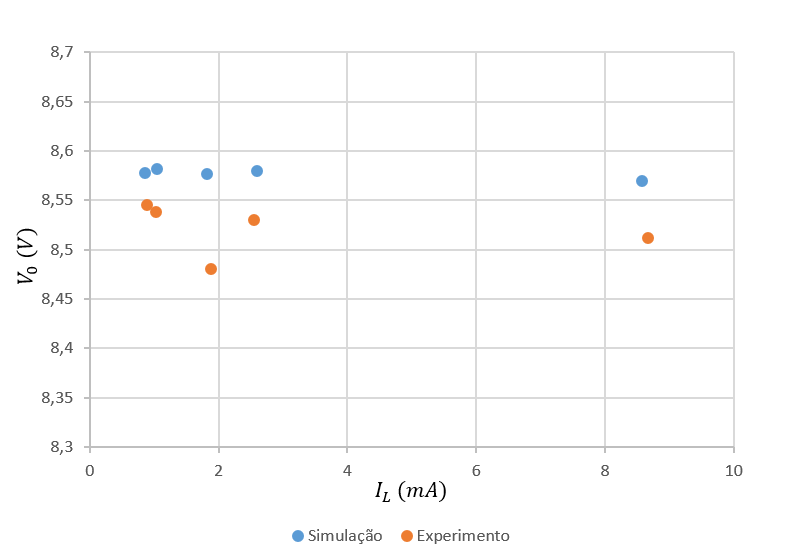
\includegraphics[width=\columnwidth]{Curva_exercicio1.png}
    		\caption{V\textsubscript{0} versus I\textsubscript{L}, com os dados da Tabela \ref{Tabela1}}
		    \label{curva1}
		    \end{center}
	    \end{figure}
	    
   \tab Espera-se que relação entre V\textsubscript{0} e I\textsubscript{L} seja dada por uma reta. Observa-se tal relação na Figura \ref{curva1}.
   
   \tab Notam-se distorções na curva experimental. No entanto, perturbações são esperadas quando se trata de experimentos. 
   
   \tab Portanto, observa-se que a simulação e o experimento estão de acordo. 
\\~\\    
    2) 
\\~\\    
         \begin{figure}[H]
		    \begin{center}
		    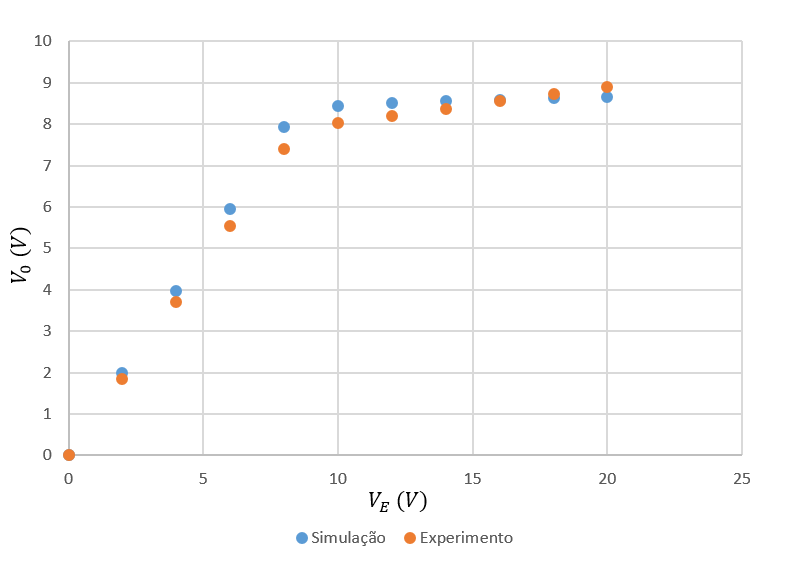
\includegraphics[width=\columnwidth]{Curva_exercicio2.png}
    		\caption{V\textsubscript{0} versus V\textsubscript{E}, com os dados da Tabela \ref{Tabela2}}
		    \label{curva2}
		    \end{center}
	    \end{figure}
    
    \tab Observa-se que ambas as curvas estão consistentes com o esperado pela teoria. Além disso, as curvas da Figura \ref{curva2} reforçam os cálculos obtidos no item 5 da seção \textbf{Exercícios}.  
\\~\\    
    3)
\\~\\

    \tab Inicialmente, necessita-se calcular a resistência interna do diodo para as condições dadas no circuito.
    
    \tab Das Figuras \ref{scope_capacitor} e \ref{scope_resistor} tem-se que, V\textsubscript{C(méd)} = 14,154 V e V\textsubscript{0(méd)} = 8,572 V. 
   
    \tab Assim, 
        \begin{equation}
            I\textsubscript{S} = \frac{ V\textsubscript{C}-  V\textsubscript{0}}{ R\textsubscript{S}} = \frac{5,582}{82} \approx 68 \: mA.
        \end{equation}
    
    Além disso, tem-se que,
        \begin{equation}
             I\textsubscript{Z} = I\textsubscript{S} - I\textsubscript{R} = I\textsubscript{S} - \frac{V\textsubscript{0}}{R\textsubscript{L}} = 59,353 \: mA
        \end{equation}
    e
        \begin{equation}
            r\textsubscript{z} = \frac{V\textsubscript{0}}{I\textsubscript{Z}} = 144,42 \: \Omega.
        \end{equation}
        
    \tab A partir do valor de r\textsubscript{z}, calcula-se o valor da resistência de Thevenin vista pelos terminais do capacitor. 
    
    Calcula-se
        \begin{equation}
            R\textsubscript{TH} = \: r\textsubscript{z}//R\textsubscript{TH} + R\textsubscript{S} = 208,19 \: \Omega.
        \end{equation}
    Finalmente, obtém-se o valor da tensão de \textit{ripple} sobre o capacitor por meio da expressão: 
        \begin{equation}
            V\textsubscript{r} = \frac{V\textsubscript{C(pico)}}{2fCR\textsubscript{TH}} = 0,56 \: V.
        \end{equation}
        
    \tab Nota-se que, ao comparar o valor de \textit{ripple} calculado acima com os valores mostrados nas Figuras \ref{V_capacitor_ripple} e \ref{scope_capacitor} (0,53 V e 0,479 V respectivamente), percebe-se que o valor está condizente com a simulação e a prática.  
    
    \tab Vale ressaltar que, tendo em vista a coerência entre cálculos teóricos, prática e simulação, necessitou-se de uma abordagem diferente quanto ao modelo equivalente do diodo zener.   
\\~\\
\\~\\
    4)
\\~\\
    
   \tab A partir do datasheet do diodo zener, tem-se que:
    
            \begin{equation}\label{datasheet zener}
        \left\{\begin{array}{ccl}
        \ V\textsubscript{Z}&=&8,2 \:V\\
        \  I\textsubscript{zk}&=&0,5 \:mA\\
        \  r\textsubscript{z}&=&4,5 \:\Omega\\
        \ I\textsubscript{zt}&=&31 \:mA.
        \end{array}\right. 
        \end{equation}
        
        \tab Inicialmente, determina-se o valor do parâmetro V\textsubscript{Z0} do modelo do diodo zener através da equação: \begin{equation}
            V\textsubscript{Z} = V\textsubscript{Z0} + r\textsubscript{z}  I\textsubscript{zt}.
        \end{equation}
        \tab Obtendo-se  V\textsubscript{Z0} = 8,06 V.
        
        \tab Da Figura \ref{scope_capacitor} tem-se que V\textsubscript{C} = 14,154 $\pm$ 0,2395 V. Logo, o pior caso (menor corrente fornecida ao resistor  R\textsubscript{L}) ocorre quando  V\textsubscript{E} = 14,154 - 0,2395 = 13,914 V.
        
        \tab Quando o diodo opera no limite da região de ruptura,  I\textsubscript{z} =  I\textsubscript{zk} e  V\textsubscript{Z} $\cong$  V\textsubscript{Z0}.
        
        \tab Daí, tem-se que 
            \begin{equation}
                 I\textsubscript{s} = \frac{13,914 - 8,06}{82} \approx 71,4 \:mA
            \end{equation}  e 
                
             \begin{equation}
                 I\textsubscript{L} =  I\textsubscript{s} -  I\textsubscript{z} \approx 70,9\: mA.
            \end{equation}
        
        \tab Portanto, \begin{equation}
            R\textsubscript{L(mín)} = \frac{8,06}{70,9 \times 10\textsuperscript{-3}} \approx 113,68 \: \Omega.
        \end{equation} 
\\~\\    
    5)
\\~\\
    \paragraph{V\textsubscript{E(mín)}}
\\~\\    
    \tab Quando o diodo zener opera em condições mínimas, tem-se que:
     
         \begin{equation}\label{condições mínimas zener}
            \left\{\begin{array}{cccl}
            \ V\textsubscript{0}&\cong&V\textsubscript{Z0}&=8,06\: V\\
            \  I\textsubscript{Z}&=&I\textsubscript{zk}&=0,5 \: mA.
            \end{array}\right. 
            \end{equation}
    \tab Daí, calcula-se: 
        \begin{equation}
            I\textsubscript{L} = \frac{V\textsubscript{0}}{10\textsuperscript{3}} = 8,06 \:mA
        \end{equation}
    e 
        \begin{equation}
            I\textsubscript{s} = I\textsubscript{Z} + I\textsubscript{L} = 8,56\: mA.
        \end{equation}
    Finalmente, 
        \begin{equation}
            V\textsubscript{E(mín)} = I\textsubscript{S} \times R\textsubscript{S} + V\textsubscript{0} = 8,762 \:V.
        \end{equation}
\\~\\    
    
    \paragraph{V\textsubscript{E(máx)}}
\\~\\
     \tab Quando o diodo zener opera em condições máximas, tem-se que:
     
         \begin{equation}\label{condições máximas zener}
            \left\{\begin{array}{cccl}
            \ I\textsubscript{Z}&=&\frac{P}{V\textsubscript{Z}}&=121,95 \: mA\\
            \ V\textsubscript{0}&=&V\textsubscript{Z0} + I\textsubscript{Z} \times r\textsubscript{z}&=8,61 \:V.
            \end{array}\right. 
            \end{equation}
    \tab Daí, calcula-se: 
         \begin{equation}
            I\textsubscript{L} = \frac{V\textsubscript{0}}{10\textsuperscript{3}} = 8,61 \:mA
        \end{equation}
    e 
        \begin{equation}
            I\textsubscript{s} = I\textsubscript{Z} + I\textsubscript{L} = 130,56 \:mA.
        \end{equation}
    Finalmente, 
        \begin{equation}
            V\textsubscript{E(máx)} = I\textsubscript{S} \times R\textsubscript{S} + V\textsubscript{0} = 19,316 \:V.
        \end{equation}    
    
\end{document}